\documentclass[11pt,a4paper]{article}
\usepackage[T1]{fontenc}
\usepackage[utf8]{inputenc}
\usepackage{lmodern}
\usepackage[margin=22mm,headheight=16pt]{geometry}
\usepackage{amsmath,amssymb,graphicx,array,longtable,booktabs}
\usepackage{microtype,xcolor,hyperref,xurl,fancyhdr}
\definecolor{Navy}{HTML}{17324D}
\definecolor{Teal}{HTML}{087F8C}
\definecolor{Gold}{HTML}{B88128}
\hypersetup{colorlinks=true,linkcolor=Navy,urlcolor=Teal,bookmarksnumbered=true,hypertexnames=false}
\setlength{\parindent}{0pt}
\setlength{\parskip}{6pt}
\setlength{\emergencystretch}{4em}
\setcounter{tocdepth}{1}
\pagestyle{fancy}\fancyhf{}
\fancyfoot[R]{\small\thepage}
\fancyfoot[L]{\small\sffamily Sharif University of Technology}
\renewcommand{\headrulewidth}{0.3pt}
\makeatletter
\renewcommand\section{\@startsection{section}{1}{\z@}{-3.2ex plus -1ex minus -.2ex}{1.6ex plus .2ex}{\normalfont\Large\sffamily\bfseries\color{Navy}}}
\renewcommand\subsection{\@startsection{subsection}{2}{\z@}{-2.5ex plus -1ex minus -.2ex}{1.2ex plus .2ex}{\normalfont\large\sffamily\bfseries\color{Teal}}}
\makeatother
\fancyhead[L]{\small\sffamily Reza Sanaee Nezhad}\fancyhead[R]{\small\sffamily Technical Report}\begin{document}
\begin{titlepage}\centering\vspace*{7mm}

\includegraphics[width=31mm]{assets/sharif_emblem_en.png}\par\vspace{5mm}
{\Large\sffamily\bfseries\color{Navy}SHARIF UNIVERSITY OF TECHNOLOGY\par}
\vspace{3mm}{\sffamily Department of Electrical Engineering\par}
\vspace{18mm}{\color{Teal}\rule{\linewidth}{1.4pt}}\par\vspace{6mm}
{\large\sffamily\color{Teal}TECHNICAL REPORT\par}
\vspace{9mm}{\huge\sffamily\bfseries\color{Navy}Coverage-Driven Verification of a Multi-Cycle ALU\par}
\vspace{10mm}{\color{Gold}\rule{45mm}{1pt}}\par\vfill
\begin{minipage}{.88\linewidth}{\sffamily\color{Teal}AUTHOR}\par{\Large\sffamily Reza Sanaee Nezhad}\par Student ID: 401101502\par\vspace{9mm}
{\sffamily\color{Teal}INSTRUCTOR}\par
Not identified in the supplied materials\par
\end{minipage}\vfill\end{titlepage}
\tableofcontents\clearpage
\section{Scope and verification architecture}

This project develops a class-based SystemVerilog verification environment for a supplied multi-cycle arithmetic logic unit. It adapts interfaces, transactions, driver, monitors, reference model, scoreboard, coverage and test selection to a packetized operand/\allowbreak{}result protocol. The environment uses mailboxes and events rather than the UVM library. The supplied RTL and framework headers credit Alireza Abbasian;\allowbreak{} the verification project and its report are by Reza Sanaee Nezhad.


An input transaction represents a complete operation and two full operands. The driver transmits that transaction as a sequence of bus-width chunks. The input monitor reconstructs accepted chunks independently and passes the complete transaction to the reference model. The output monitor collects result chunks or reset notifications. The scoreboard checks them against the reference queue and distinguishes completed results from operations canceled by a legal reset. Functional covergroups connect the tests to a spreadsheet-style plan.

\begin{figure}[!htbp]\centering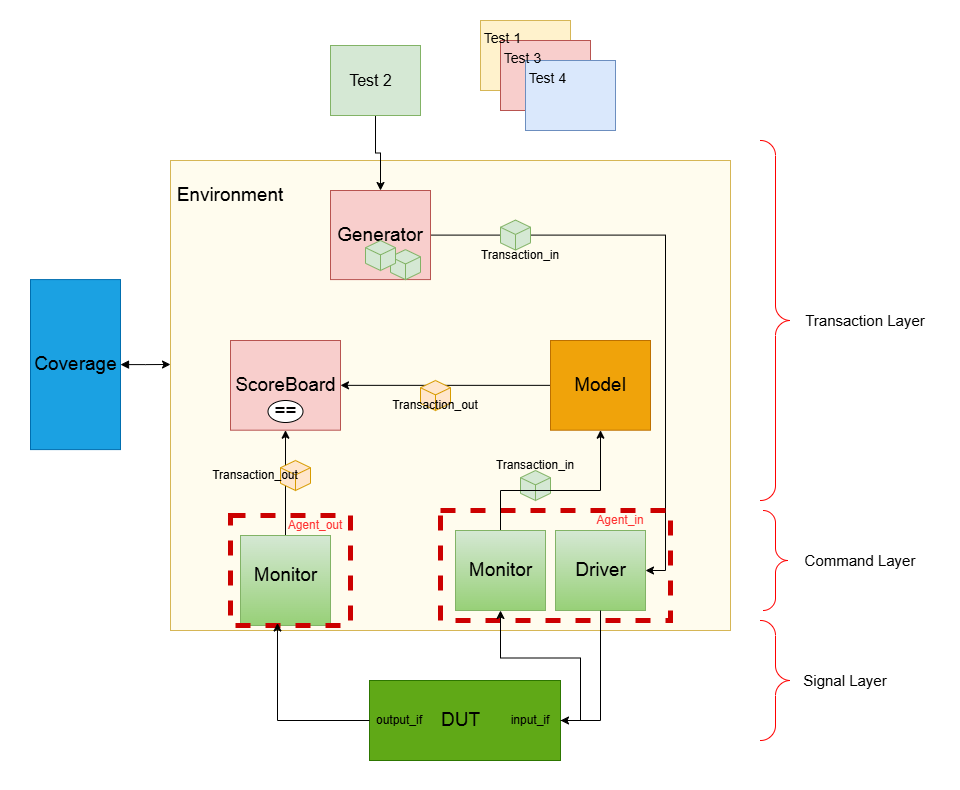
\includegraphics[width=\linewidth,height=.70\textheight,keepaspectratio]{assets/systemverilog_verification_flow.png}\caption{Supplied verification architecture: generator, driver, input/output monitors, reference model, scoreboard and coverage.}\end{figure}
\clearpage
\section{Parameters and operation contract}

The default operand bus width is eight bits and each complete unsigned operand is 32 bits. The result bus is 16 bits and complete result storage is 64 bits. A complete operand pair therefore uses four accepted input beats. Results are sent least-significant chunk first, using one to four beats as indicated by result\_\allowbreak{}last. A zero or sufficiently small result uses one beat. The monitor reconstructs the complete result in initially zeroed storage, so omitted leading zero chunks do not leave stale data.


The physical rst input is active low. Software reset is opcode 111 with operand\_\allowbreak{}valid asserted, and it is accepted even while ready is low. The normal opcodes are no-op 000, unsigned addition 001, bitwise AND 010, bitwise XOR 011 and unsigned multiplication 100. Opcodes 101 and 110 are excluded by the transaction constraint and classified as illegal coverage bins. No-op does not generate an arithmetic output transaction. Software reset clears result storage, deasserts result\_\allowbreak{}valid, asserts result\_\allowbreak{}rst and returns the unit to IDLE.


The RTL uses IDLE, RECEIVE, EXECUTE and SEND states. ready is asserted in IDLE and RECEIVE. Arithmetic uses the operation captured with the first operand beat. Operand widths must divide the full operand width, result bus width must divide the full result width, and the result width must accommodate the complete unsigned product. Parameter checks reject unsupported configurations. The result bus has one combinational writer driven from the full-result register and chunk index.

\begingroup\small\setlength{\tabcolsep}{4pt}\renewcommand{\arraystretch}{1.22}\begin{longtable}{@{}p{0.12\linewidth}p{0.27\linewidth}p{0.52\linewidth}@{}}
\caption{Legal operation semantics}\\\toprule
\textbf{Opcode} & \textbf{Operation} & \textbf{Output reference} \\ \midrule\endfirsthead \textbf{Opcode} & \textbf{Operation} & \textbf{Output reference} \\ \midrule\endhead
000 & No-op & No arithmetic result \\
001 & Unsigned add & Extended a+b \\
010 & Bitwise AND & a \& b \\
011 & Bitwise XOR & a XOR b \\
100 & Unsigned multiply & Full a*b \\
111 & Software reset & Zero; result\_rst=1 \\
\bottomrule\end{longtable}\endgroup
\clearpage
\section{Input and output interfaces}

The input interface carries ready, operand\_\allowbreak{}valid, operand\_\allowbreak{}last, op, a and b together with clock and active-low reset. Its DUT modport receives the operand and control signals and produces ready. The driver modport drives operands and control while observing ready, clock and reset. The monitor modport observes all signals without driving them. Distinguishing these directions makes the interaction between the three roles explicit.


The output interface carries result\_\allowbreak{}valid, result\_\allowbreak{}last, result\_\allowbreak{}rst and the result chunk. The DUT drives these signals, and the monitor observes them. The top-level module connects the four width parameters and every input/\allowbreak{}output control signal to the corresponding DUT port. Both interfaces share the same system clock and physical reset.

\begin{figure}[!htbp]\centering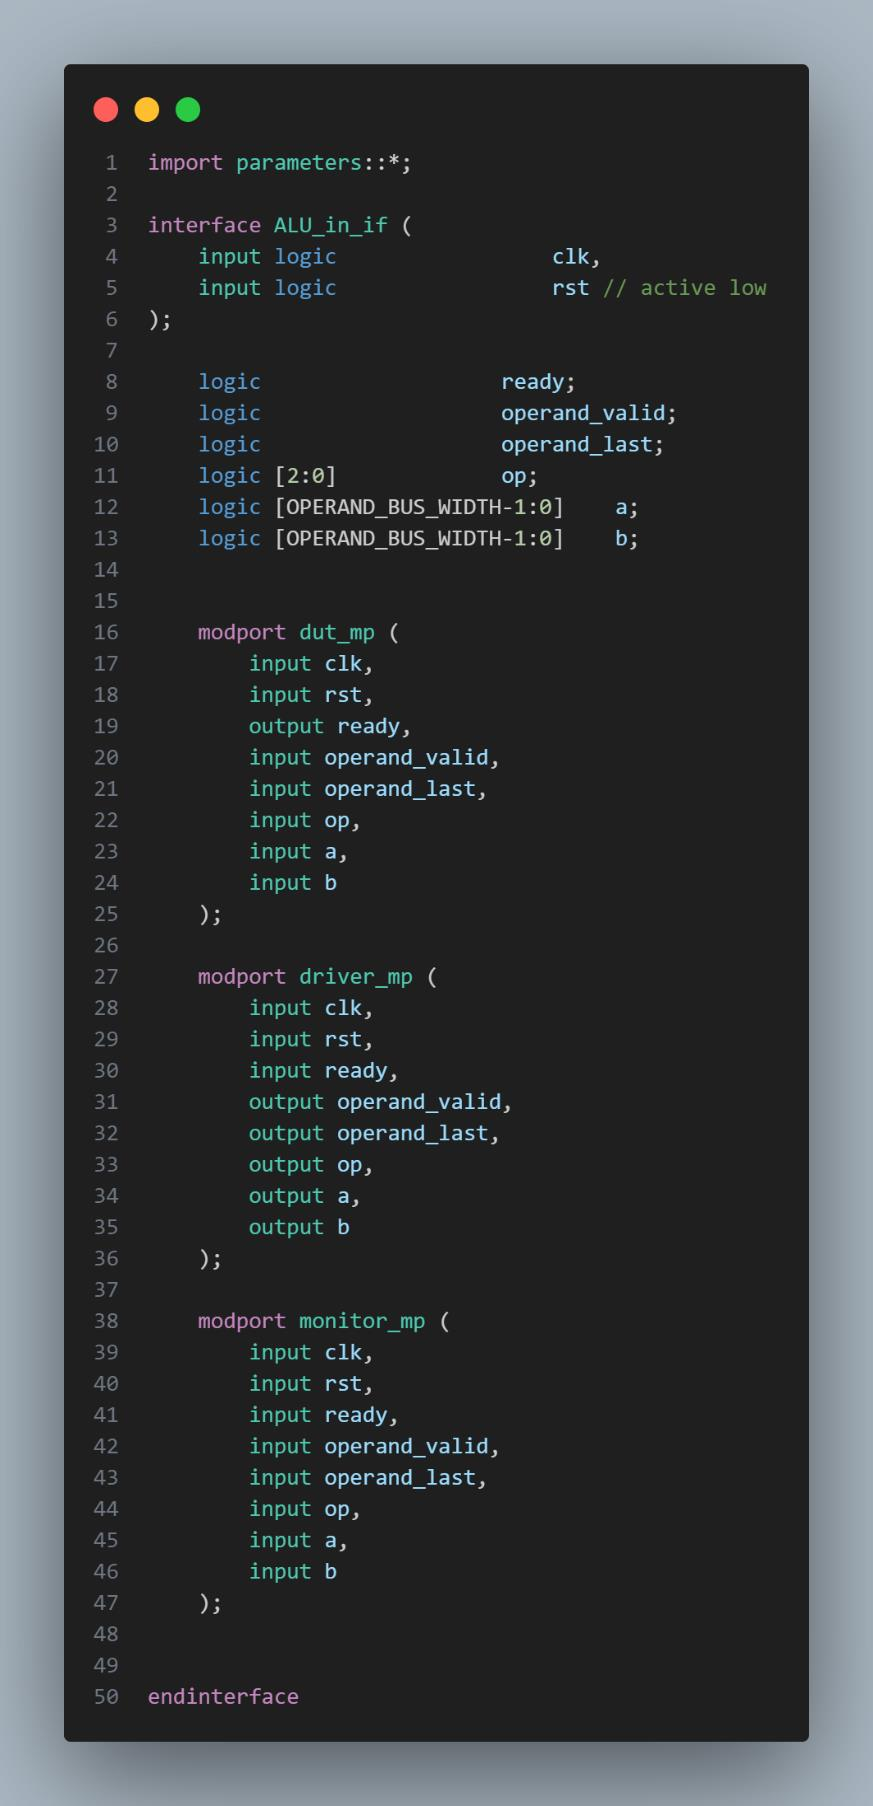
\includegraphics[width=\linewidth,height=.70\textheight,keepaspectratio]{assets/p02_25.jpeg}\caption{Input interface and direction-specific modports.}\end{figure}
\begin{figure}[!htbp]\centering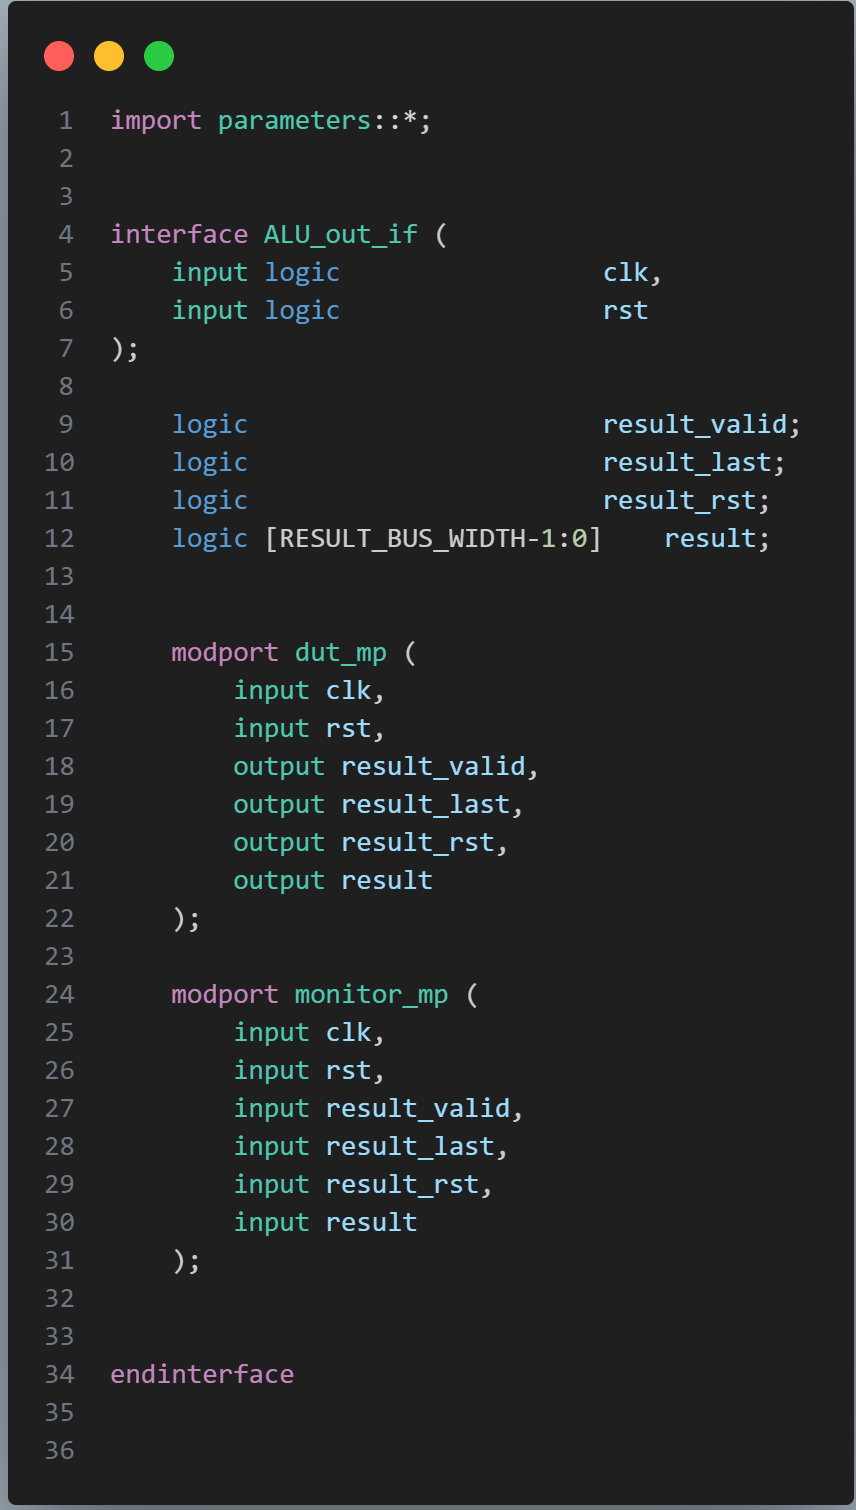
\includegraphics[width=\linewidth,height=.70\textheight,keepaspectratio]{assets/p03_23.png}\caption{Output interface and observer modport.}\end{figure}
\clearpage
\section{Input transactions, constraints and copying}

ALU\_\allowbreak{}in\_\allowbreak{}transaction contains a randomized operation, full-width a and b values, and the four-bit randomized clk\_\allowbreak{}gap. Its legal-operation constraint permits the six defined opcodes. Its gap constraint permits values zero through fourteen inclusive. clk\_\allowbreak{}gap specifies ready idle cycles before starting a normal operand frame;\allowbreak{} it does not represent the total latency of a previous operation or clocks spent waiting for ready.


The input transaction stores all 32 bits of each operand even though the bus carries eight bits at a time. Serialization belongs to the driver rather than to the generator. do\_\allowbreak{}copy copies op, a, b and clk\_\allowbreak{}gap into a separate object. do\_\allowbreak{}compare compares operation and operand values;\allowbreak{} timing gap is excluded because two transactions with identical arithmetic inputs can have different idle spacing without changing the mathematical result.


ALU\_\allowbreak{}in\_\allowbreak{}transaction\_\allowbreak{}range extends the base transaction with inclusive minimum and maximum bounds for each operand. Randomization obeys both the inherited legal-operation/\allowbreak{}gap constraints and the range constraints. Its copy method retains the range bounds and clk\_\allowbreak{}gap as well as arithmetic fields. Range display uses inclusive endpoints, matching the actual greater-than-or-equal and less-than-or-equal constraints.

\begin{figure}[!htbp]\centering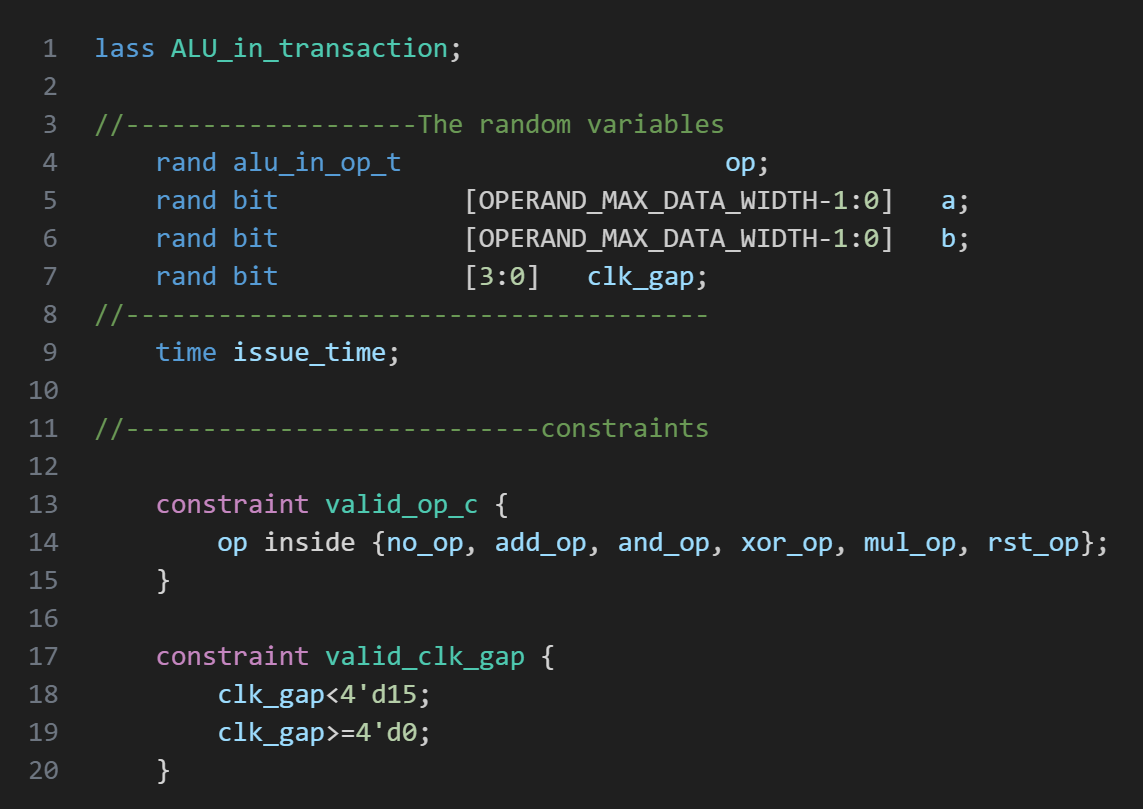
\includegraphics[width=\linewidth,height=.70\textheight,keepaspectratio]{assets/p04_21.png}\caption{Full-width randomized operands and constrained idle gap.}\end{figure}
\begin{figure}[!htbp]\centering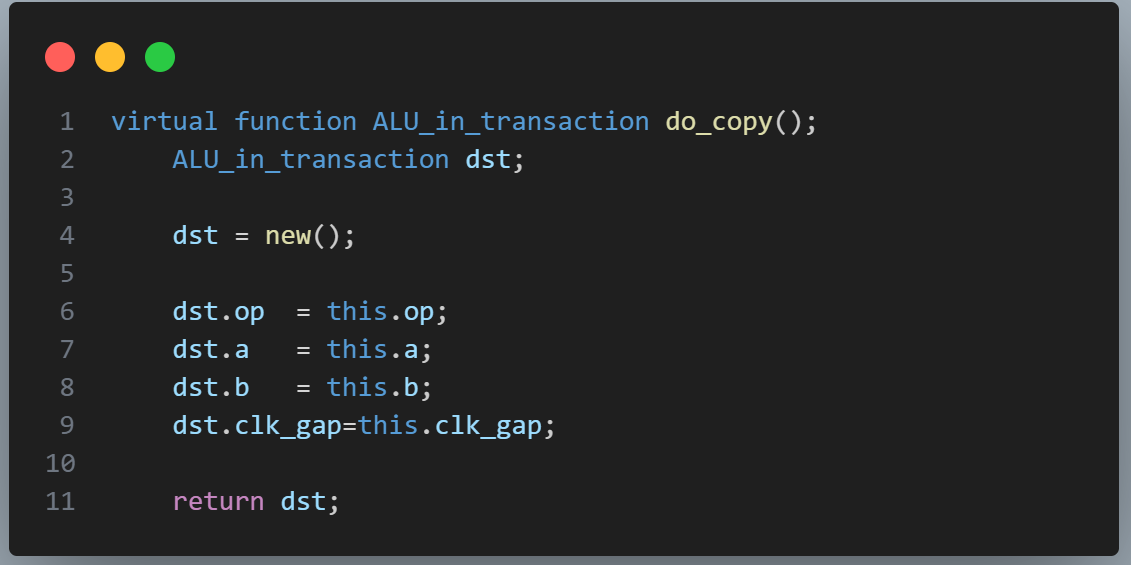
\includegraphics[width=\linewidth,height=.70\textheight,keepaspectratio]{assets/p05_24.png}\caption{Input transaction copying includes clk\_gap.}\end{figure}
\clearpage
\section{Output transactions and interruption state}

ALU\_\allowbreak{}out\_\allowbreak{}transaction stores the complete 64-bit result, result\_\allowbreak{}rst, an aborted flag and an issue timestamp. A new object initializes interruption state to false, and complete reconstruction starts with zeroed result storage. The copy method retains result, reset flag and interruption state in a separate object. Its arithmetic comparison checks result and result\_\allowbreak{}rst.


The aborted flag means a pending arithmetic operation was interrupted by a software reset. It is not an alternative successful arithmetic result. In that event the observable reset output must be zero and must have result\_\allowbreak{}rst asserted. The canceled arithmetic operation and the completed reset command are accounted for separately. This prevents a flagged result from being accepted merely because its interruption bit is set.

\section{Driver scheduling and packet serialization}

The generator sends transaction objects through gen2drv. The driver removes one object, transmits it, and signals drv2gen so that generation can continue. Stimulus is driven on falling clock edges and accepted by the DUT on rising edges. This places values on the bus before the DUT's sampling edge rather than changing them in the same active event region as DUT sampling.


For a normal transaction, the driver waits until the physical reset is released and ready is asserted. It waits the requested number of ready idle clocks, then sends four successive eight-bit portions from a and b. The indexed slice for beat i begins at bit i*OPERAND\_\allowbreak{}BUS\_\allowbreak{}WIDTH. operand\_\allowbreak{}valid is asserted for each beat, and operand\_\allowbreak{}last is asserted only for the final beat. After the last accepted beat, the control signals are deasserted on a falling edge. The full operand object is not modified by serialization.


For software reset, the driver waits for physical reset release but does not wait for ready. It asserts operand\_\allowbreak{}valid with rst\_\allowbreak{}op for one accepted cycle. This enables a reset command during calculation or result collection, when the unit is busy. Consecutive software-reset commands remain separate accepted commands even when result\_\allowbreak{}rst is asserted in consecutive cycles. Generator/\allowbreak{}driver event synchronization prevents two threads from driving competing operand frames.

\section{Input monitor and observed idle gap}

The input monitor samples at rising edges, when the driver values are stable. An ordinary accepted beat requires operand\_\allowbreak{}valid and ready while physical reset is released. A reset command can be recognized with operand\_\allowbreak{}valid and rst\_\allowbreak{}op even when ready is low. The monitor creates a new transaction at the start of an accepted frame and records the operation from the bus rather than from the driver's object.


For an ordinary frame, each accepted eight-bit a and b chunk is placed at its corresponding position in the 32-bit transaction. The monitor continues until operand\_\allowbreak{}last and checks that the frame cannot exceed the declared maximum number of beats. A gap between beats is not filled with unaccepted bus data. The reconstructed object is copied into the model mailbox only after the frame has completed.


Idle-cycle counting includes ready clocks without a valid new operand, and excludes busy clocks and physical-reset time. The observed gap is checked against the zero-to-fourteen stimulus contract before assignment to the four-bit field. A software-reset input produces a reset transaction directly. Input functional coverage is sampled from monitored transactions, so it reflects accepted bus behavior rather than requested generator values.

\section{Output monitor and reset event capture}

The output monitor samples on falling edges, after the DUT's rising-edge updates have settled. It waits until the physical reset is released and either result\_\allowbreak{}valid or result\_\allowbreak{}rst is asserted. A result transaction is reconstructed from successive 16-bit chunks in 64-bit storage. result\_\allowbreak{}last identifies the final chunk, and the monitor checks the maximum beat count.


If result\_\allowbreak{}valid disappears before result\_\allowbreak{}last without a reset notification, the monitor reports a protocol failure. If result\_\allowbreak{}rst arrives during reconstruction, the partial numeric value is not treated as a valid completed answer;\allowbreak{} the record contains a zero reset result and is marked as interrupted. A reset arriving before the first result beat is also emitted as a reset record and is associated with the pending arithmetic reference by the scoreboard.


One software-reset record is emitted per active reset cycle. The next monitor call starts at the next falling edge. This allows two back-to-back accepted reset commands to be observed separately. Physical-reset cycles are excluded while rst is low. The stream is therefore not collapsed into one event merely because result\_\allowbreak{}rst remains high across adjacent command cycles.

\section{Reference model}

The model receives independently monitored full input transactions. Addition produces an unsigned extended sum in result-width storage, AND and XOR produce their bitwise results, and multiplication produces the complete unsigned product. Ordinary arithmetic results have result\_\allowbreak{}rst equal to zero. rst\_\allowbreak{}op produces a zero result with result\_\allowbreak{}rst equal to one. No-op produces no expected arithmetic result and is not enqueued into the output reference stream.


The model does not use the randomized idle gap in calculation. Time spacing influences protocol execution and coverage, but not arithmetic. A mailbox carries expected result objects to the scoreboard in accepted transaction order. The operation/\allowbreak{}result mapping is shown in the table and reference-model implementation.

\begin{figure}[!htbp]\centering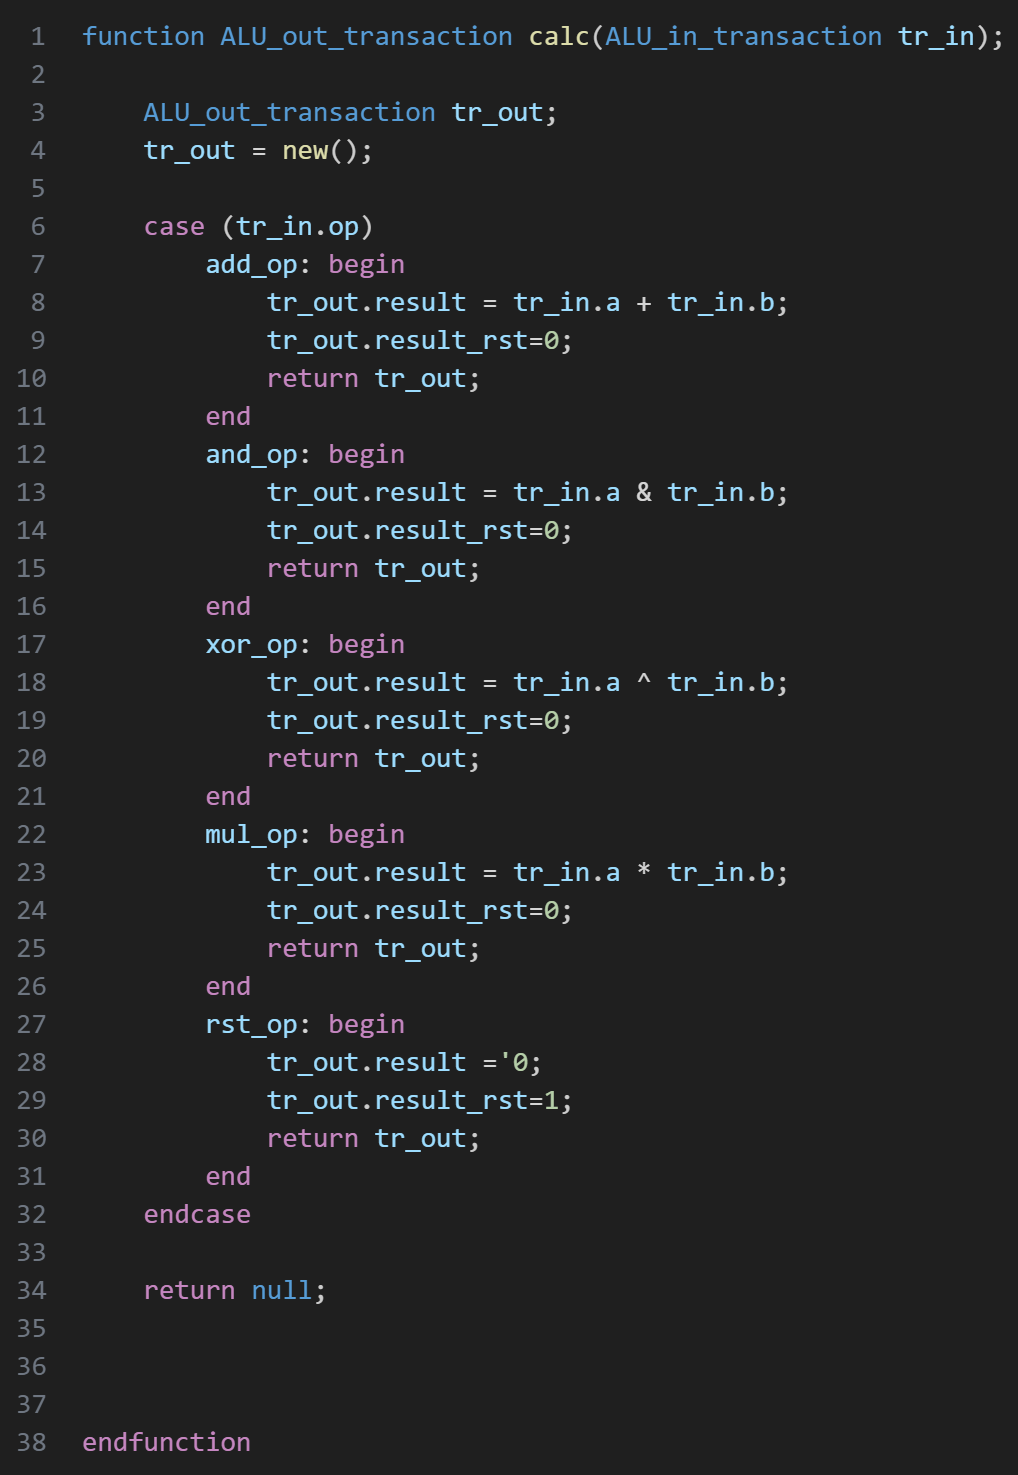
\includegraphics[width=\linewidth,height=.70\textheight,keepaspectratio]{assets/p14_23.png}\caption{Arithmetic and software-reset reference calculation.}\end{figure}
\clearpage
\section{Scoreboard ordering and legal cancellation}

The scoreboard consumes expected and actual records in order. A complete ordinary result must match both numeric result and reset flag. A clean reset result must match the reset reference. A mismatch increments the failed count and prints both objects;\allowbreak{} a nonzero failed count terminates the test as a failure.


When an actual reset arrives while the next expected record is an arithmetic result, the reset legally cancels that pending operation. The observable result must still be zero. The scoreboard increments a separate aborted counter and consumes the following reset reference to check the actual reset notification. It does not count the canceled arithmetic operation as a passed result. Unexpected reset behavior cannot silently pass because the following expected record must also compare as a reset.


Output functional coverage is sampled after this classification, so interruption coverage includes a reset before the first result beat as well as during result collection. The canceled operation and completed reset command are represented separately for coverage accounting without placing duplicate physical output records in the mailbox. The final summary reports passed, aborted and failed counts, and both remaining queue sizes. The automated runner requires zero failures and no pending records.

\section{Testbench integration and test profiles}

The top-level testbench starts with physical reset asserted, releases it after 200 ns, and generates a clock that toggles every 5 ns, for a 10 ns period. Interfaces and the DUT share that clock. Compile-time test selection chooses random\_\allowbreak{}test, test\_\allowbreak{}mid, test\_\allowbreak{}high or test\_\allowbreak{}mix. The selected name is also recorded in the coverage database so that labels agree with the instantiated test.


random\_\allowbreak{}test uses the complete legal operand space. test\_\allowbreak{}mid uses explicit width-safe bounds from the midpoint through the maximum unsigned operand. test\_\allowbreak{}high restricts operands to the largest two representable values. test\_\allowbreak{}mix successively uses unrestricted, mid-range, high-range and low-range profiles. Range endpoints are inclusive. A selected blueprint is installed before generation begins. Reset/\allowbreak{}no-op operand defaults are not counted as numeric operand coverage.


The mid and high tests run for 20000 ns;\allowbreak{} the mixed profile runs through its successive timed phases, and the random test runs for approximately 100000 ns. Each environment includes generator, driver, model, input monitor, output monitor and scoreboard threads. Tests terminate with a scoreboard summary rather than relying on an infinite background clock to stop by itself.

\begin{figure}[!htbp]\centering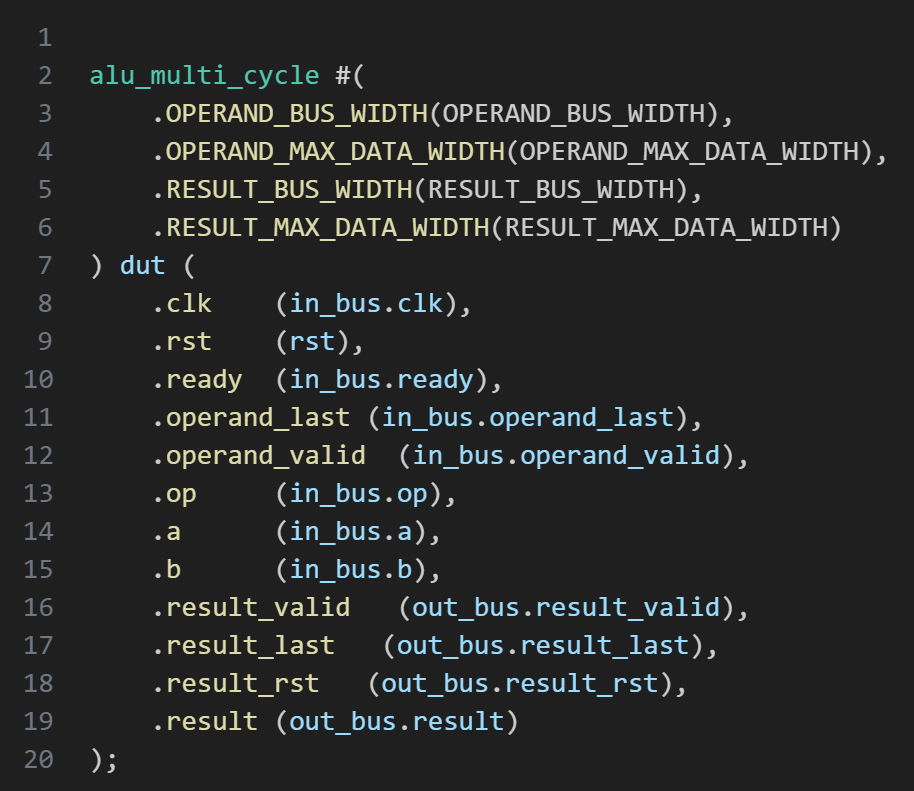
\includegraphics[width=\linewidth,height=.70\textheight,keepaspectratio]{assets/p15_26.png}\caption{Width parameters and DUT port connections.}\end{figure}
\clearpage
\section{Functional coverage and complete test plan}

The input operation coverpoint has six legal bins and default illegal bins for undefined opcodes. Each legal bin requires at least ten hits. Operand coverpoints are sampled only for add, AND, XOR and multiply operations. For 32-bit unsigned operands, low covers zero through 0x7fffffff, mid covers 0x80000000 through 0xfffffffd, and high covers 0xfffffffe through 0xffffffff. These three ranges are disjoint and include both endpoint values.


The idle-gap coverpoint excludes reset commands and has three bins:\allowbreak{} zero, one through eight, and nine through fourteen. The three groups match the constrained input domain. Fifteen is not a legal requested gap. The input group contains fifteen bins:\allowbreak{} six operation bins, three a bins, three b bins and three gap bins.


The output numeric result is covered only when the record is neither a reset nor an aborted operation. Its two bins span zero through 0x7fffffffffffffff and 0x8000000000000000 through 0xffffffffffffffff. result\_\allowbreak{}rst has zero and one bins. reset\_\allowbreak{}during\_\allowbreak{}calculation has noninterrupted and interrupted bins. The output group contains six bins, giving twenty-one defined functional bins in total. Each bin uses an at-least-ten hit goal.


The test-plan CSV links operation, a, b, gap, result, reset notification and interruption coverpoints. The input section has weight three, the output section weight one, and the operation requirement weight five. Every requirement's goal is 100 percent. The supplied workbook representation and the native plan table preserve all of these links and weights. Coverage measures exercised definitions, not the correctness of every possible input or the completeness of the definitions themselves.

\begingroup\small\setlength{\tabcolsep}{4pt}\renewcommand{\arraystretch}{1.22}\begin{longtable}{@{}p{0.21\linewidth}p{0.51\linewidth}p{0.09\linewidth}p{0.09\linewidth}@{}}
\caption{Complete spreadsheet-style coverage plan}\\\toprule
\textbf{Requirement} & \textbf{Link suffix} & \textbf{Weight} & \textbf{Goal} \\ \midrule\endfirsthead \textbf{Requirement} & \textbf{Link suffix} & \textbf{Weight} & \textbf{Goal} \\ \midrule\endhead
Input section & - & 3 & 100\% \\
Operations & ALU\_in\_transaction\_cg:op & 5 & 100\% \\
Operand A & ALU\_in\_transaction\_cg:a & 1 & 100\% \\
Operand B & ALU\_in\_transaction\_cg:b & 1 & 100\% \\
Clock gap & ALU\_in\_transaction\_cg:clk\_gap & 1 & 100\% \\
Output section & - & 1 & 100\% \\
Result & ALU\_out\_transaction\_cg:result & 1 & 100\% \\
Reset observed & ALU\_out\_transaction\_cg:result\_rst & 1 & 100\% \\
Reset interruption & ALU\_out\_transaction\_cg:reset\_during\_calculation & 1 & 100\% \\
\bottomrule\end{longtable}\endgroup
\begin{figure}[!htbp]\centering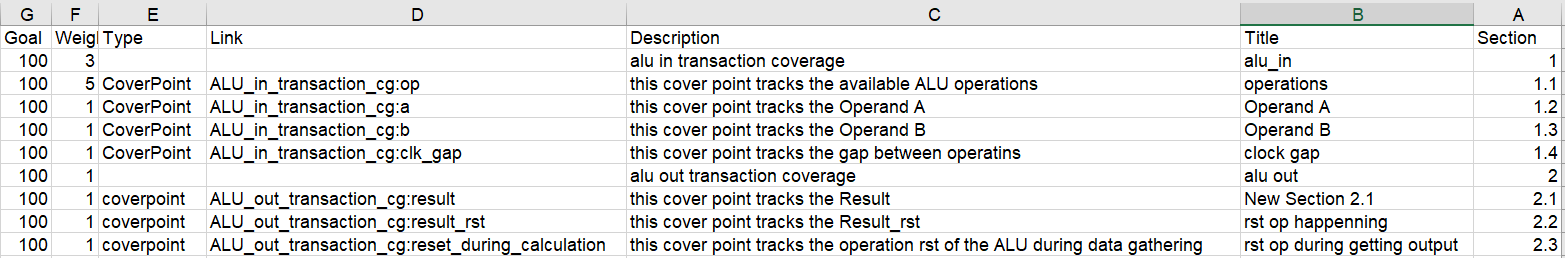
\includegraphics[width=\linewidth,height=.70\textheight,keepaspectratio]{assets/p17_23.png}\caption{Spreadsheet representation in the recorded academic report.}\end{figure}
\clearpage
\section{Recorded academic coverage and ranking figures}

The recorded classroom report contains a Questa HTML summary with two tests marked OK, a weighted test-plan total of 100 percent, and twenty-one bins shown as covered. The output result, result\_\allowbreak{}rst and reset\_\allowbreak{}during\_\allowbreak{}calculation displays each show two covered bins and no missing bins. These figures are retained as the academic experiment record, together with the original spreadsheet and rank summaries.


One captured ranking lists test\_\allowbreak{}mid42 with total coverage 88.06 percent and test-plan coverage 93.75 percent. The other lists test\_\allowbreak{}high42 with total coverage 87.46 percent and test-plan coverage 100 percent. Both captured summaries report 0.06 seconds of CPU time;\allowbreak{} their simulation-time entries are 20050000 ps and 20000000 ps respectively. These are different reported metrics and captured views. A 100-percent test-plan goal is not the same quantity as the total-coverage percentage, and the two screenshots do not demonstrate monotonic aggregate coverage between two database merges.


Zero operand values associated with reset/\allowbreak{}no-op transactions do not establish that a numeric low-range test has been exercised. The arithmetic operand coverpoints therefore use the operation qualification described above. The ranking objective is to identify a small useful set of tests against defined coverage goals, rather than infer correctness from a high percentage alone.

\begin{figure}[!htbp]\centering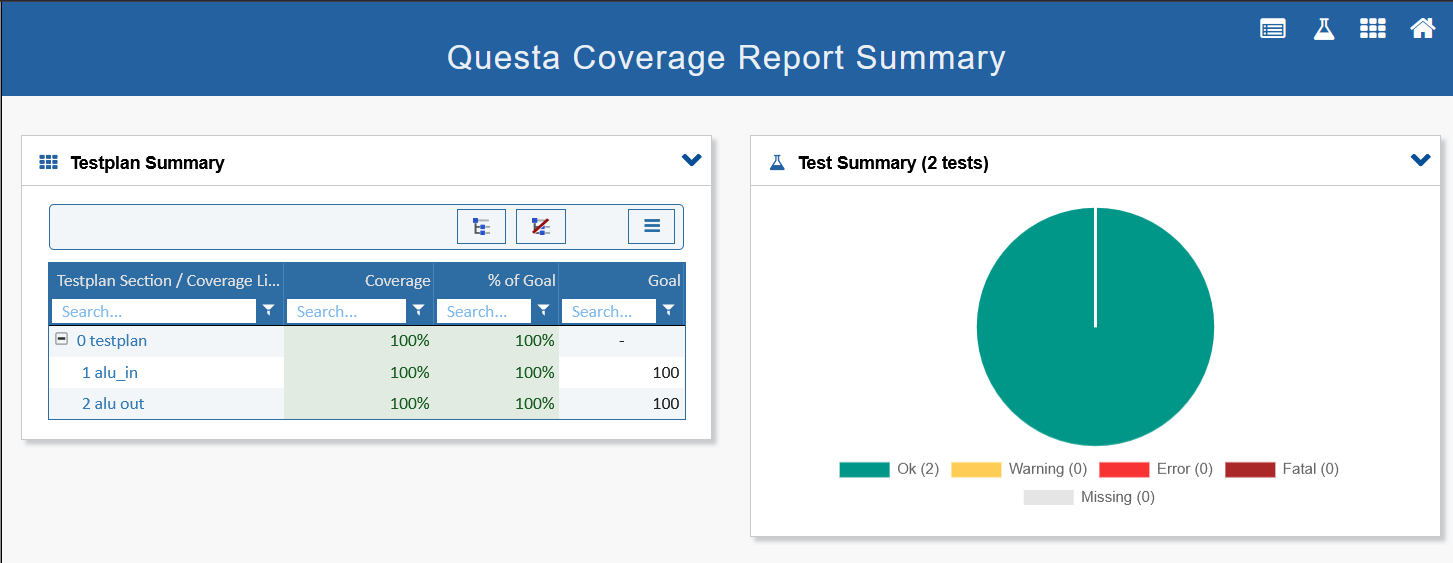
\includegraphics[width=\linewidth,height=.70\textheight,keepaspectratio]{assets/p18_06.png}\caption{Recorded Questa test-plan summary and two-test status.}\end{figure}
\begin{figure}[!htbp]\centering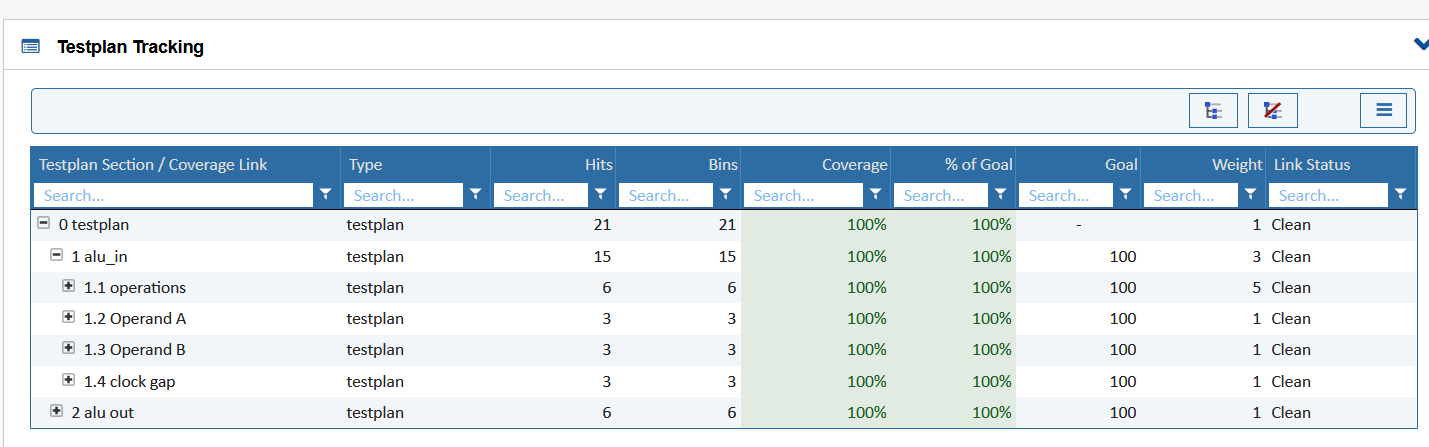
\includegraphics[width=\linewidth,height=.70\textheight,keepaspectratio]{assets/p18_07.png}\caption{Recorded test-plan tracking view with twenty-one functional bins.}\end{figure}
\begin{figure}[!htbp]\centering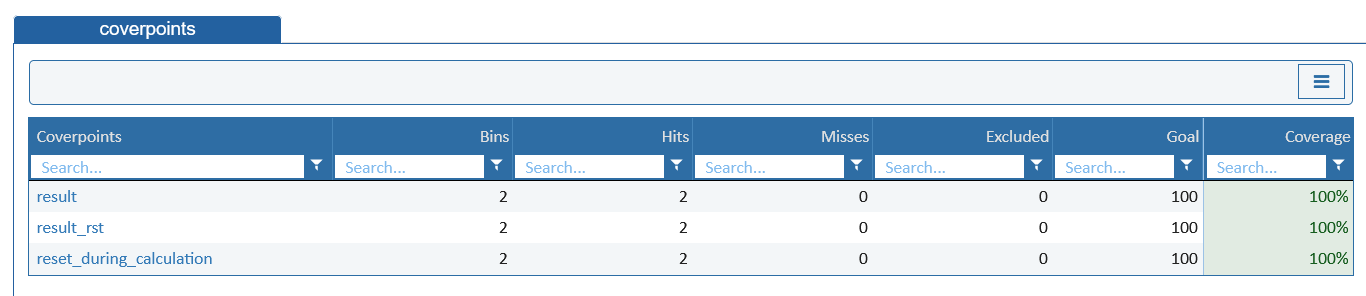
\includegraphics[width=\linewidth,height=.70\textheight,keepaspectratio]{assets/p18_08.png}\caption{Recorded output coverpoints: result, reset and interruption.}\end{figure}
\begin{figure}[!htbp]\centering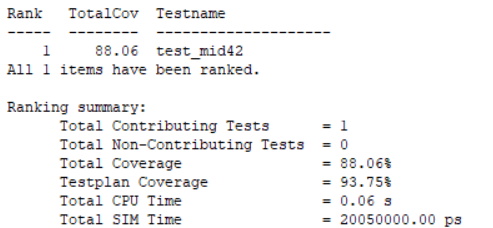
\includegraphics[width=\linewidth,height=.70\textheight,keepaspectratio]{assets/p19_19.png}\caption{Captured academic ranking output for test\_mid42.}\end{figure}
\begin{figure}[!htbp]\centering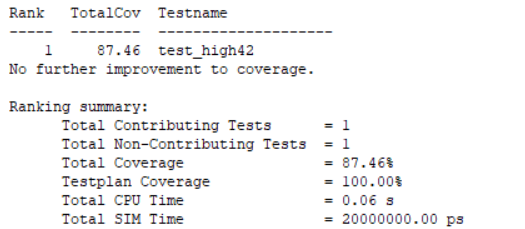
\includegraphics[width=\linewidth,height=.70\textheight,keepaspectratio]{assets/p19_20.png}\caption{Captured academic ranking output for test\_high42.}\end{figure}
\clearpage
\section{Reproducible simulation results}

The distributed runner compiles and elaborates each selected test using Questa 2021.1, runs it with seed 42, captures the scoreboard and saves its UCDB. Compilation and elaboration report zero errors and zero warnings for the four test profiles. The results table gives completed comparisons, legal cancellations, failures, queue sizes and functional covergroup coverage for each execution.


All four runs have zero failed comparisons and empty expected/\allowbreak{}actual queues at the end. Together they contain 1164 completed comparisons and 189 separately classified legal cancellations. Merging their functional coverage covers all twenty-one defined bins and reports 100 percent covergroup coverage. This statement is limited to the explicit functional model and hit goals;\allowbreak{} it is not a claim of complete RTL code coverage or a formal proof.


Iterative functional-coverage ranking uses the four individual databases. random\_\allowbreak{}test42 contributes a reported aggregate functional metric of 91.66 percent;\allowbreak{} adding test\_\allowbreak{}high42 reaches 100 percent. Two tests contribute and two do not add coverage under that ranking goal. The ranking summary reports 0.02 seconds of CPU time and 120050000 ps of simulation time. The decimal value printed by the ranking tool is retained rather than interpreted as an exact count fraction.

\begingroup\small\setlength{\tabcolsep}{4pt}\renewcommand{\arraystretch}{1.22}\begin{longtable}{@{}llllll@{}}
\caption{Seed-42 simulation summaries and functional covergroup coverage}\\\toprule
\textbf{Test} & \textbf{Passed} & \textbf{Aborted} & \textbf{Failed} & \textbf{Queues E/A} & \textbf{Functional} \\ \midrule\endfirsthead \textbf{Test} & \textbf{Passed} & \textbf{Aborted} & \textbf{Failed} & \textbf{Queues E/A} & \textbf{Functional} \\ \midrule\endhead
test\_mid & 132 & 18 & 0 & 0/0 & 83.33\% \\
test\_high & 133 & 19 & 0 & 0/0 & 83.33\% \\
test\_mix & 235 & 39 & 0 & 0/0 & 87.50\% \\
random\_test & 664 & 113 & 0 & 0/0 & 91.66\% \\
\bottomrule\end{longtable}\endgroup
\begingroup\small\setlength{\tabcolsep}{4pt}\renewcommand{\arraystretch}{1.22}\begin{longtable}{@{}lll@{}}
\caption{Iterative functional ranking from the individual databases}\\\toprule
\textbf{Rank} & \textbf{Test} & \textbf{Functional metric} \\ \midrule\endfirsthead \textbf{Rank} & \textbf{Test} & \textbf{Functional metric} \\ \midrule\endhead
1 & random\_test42 & 91.66\% \\
2 & test\_high42 & 100.00\% \\
\bottomrule\end{longtable}\endgroup
\clearpage
\section{Execution and engineering limits}

run.py locates Questa tools on PATH, creates a separate build library and results directory for each test/\allowbreak{}seed, compiles sources in dependency order, elaborates top, and loads the elaborated design directly in command-line mode. Relative library paths avoid legacy simulator parsing of spaces in a Windows parent directory. The runner checks diagnostic messages as well as process return codes, because a simulator can finish with a successful process code after reporting a fatal testbench failure.


The package includes the full RTL, interfaces, class environment, tests, test plan, compiled-result summaries, UCDBs and functional-coverage/\allowbreak{}ranking output. The build libraries are regenerable and are not required to inspect the project. The report does not establish FPGA placement, timing closure, power or area improvement. Verification uses a finite test set and a model;\allowbreak{} additional assertions, directed protocol cases and formal methods could expand assurance beyond the stated experiments.

\clearpage\appendix\section{Implementation details}
\subsection{ALU\_out\_transaction.sv}
\begin{figure}[!htbp]\begin{minipage}{\linewidth}\fontsize{10}{11.4}\selectfont\begin{verbatim}
//--------------------------------------
// Last Update  : 1403/3
// Author       : Alireza Abbasian
//--------------------------------------

class ALU_out_transaction;

//-------------------The random variables
    
//--------------------------------------
    time issue_time;
    bit [RESULT_MAX_DATA_WIDTH-1:0] result ;
    bit result_rst;
    bit aborted;

//---------------------------constraints

//--------------------------------------

//-----------------------------functions
    function new();

        this.issue_time = $time;
        this.aborted=0;
    endfunction 

    virtual function string convert2string();

    string string_out = "ALU_out_transaction:\n";

        string_out = {string_out, $sformatf("result:0x%x \n",result)};
        string_out = {string_out, $sformatf("result_rst= %b\n", 
    result_rst)};

        return string_out;

    endfunction

    virtual function void do_print();

        $display(convert2string());

    endfunction

    virtual function bit do_compare (input ALU_out_transaction rhs);

\end{verbatim}\end{minipage}\caption{Implementation: ALU\_out\_transaction.sv (panel 1 of 2).}\end{figure}
\begin{figure}[!htbp]\begin{minipage}{\linewidth}\fontsize{10}{11.4}\selectfont\begin{verbatim}
        return (
                 (this.result == rhs.result) && (this.result_rst == 
    rhs.result_rst)
                );

    endfunction

    virtual function ALU_out_transaction do_copy();
        ALU_out_transaction dst;

        dst = new();
        
        dst.result  = this.result;
        dst.result_rst  = this.result_rst;
        dst.aborted  = this.aborted;
        return dst;

    endfunction : do_copy

//--------------------------------------

endclass
\end{verbatim}\end{minipage}\caption{Implementation: ALU\_out\_transaction.sv (panel 2 of 2).}\end{figure}
\clearpage
\subsection{ALU\_in\_transaction\_range.sv}
\begin{figure}[!htbp]\begin{minipage}{\linewidth}\fontsize{10}{11.4}\selectfont\begin{verbatim}
//--------------------------------------
// Last Update  : 1403/3
// Author       : Alireza Abbasian
//--------------------------------------

class ALU_in_transaction_range extends ALU_in_transaction;

//--------------------------------------
     bit [OPERAND_MAX_DATA_WIDTH-1:0] a_min;
     bit [OPERAND_MAX_DATA_WIDTH-1:0] a_max;
     bit [OPERAND_MAX_DATA_WIDTH-1:0] b_min;
     bit [OPERAND_MAX_DATA_WIDTH-1:0] b_max;

//---------------------------constraints

    constraint a_range { 
        a >=    a_min; 
        a <=     a_max;
    }

    constraint b_range { 
        b >=    b_min; 
        b <=     b_max;
    }

//--------------------------------------

//-----------------------------functions
    function new();

        super.new();

    endfunction 

    virtual function string convert2string();

        string string_out = super.convert2string();
        
        string_out = {
            string_out, 
            $sformatf(
                "ranged transaction: a in [%0d,%0d], b in [%0d,%0d]\n", 
                a_min, a_max, b_min, b_max
            )
        };
        
\end{verbatim}\end{minipage}\caption{Implementation: ALU\_in\_transaction\_range.sv (panel 1 of 2).}\end{figure}
\begin{figure}[!htbp]\begin{minipage}{\linewidth}\fontsize{10}{11.4}\selectfont\begin{verbatim}
        return string_out;

    endfunction

    virtual function void do_print();

        $display(convert2string());

    endfunction

    virtual function bit do_compare (input ALU_in_transaction rhs);
        ALU_in_transaction_range rhs_range;

        // Ensure the cast is valid before proceeding
        if (!$cast(rhs_range, rhs)) begin
            return super.do_compare(rhs);
        end

        return super.do_compare(rhs_range) &&
               (this.a_min == rhs_range.a_min) &&
               (this.a_max == rhs_range.a_max) &&
               (this.b_min == rhs_range.b_min) &&
               (this.b_max == rhs_range.b_max);
    endfunction

    virtual function ALU_in_transaction do_copy();
        ALU_in_transaction_range dst;

        dst = new();
        
        dst.op     = this.op;
        dst.a      = this.a;
        dst.b      = this.b;
        dst.clk_gap = this.clk_gap;

        dst.a_min  = this.a_min;
        dst.a_max  = this.a_max;
        dst.b_min  = this.b_min;
        dst.b_max  = this.b_max;

        return dst;
    endfunction : do_copy

//--------------------------------------

endclass
\end{verbatim}\end{minipage}\caption{Implementation: ALU\_in\_transaction\_range.sv (panel 2 of 2).}\end{figure}
\clearpage
\subsection{ALU\_in\_driver.sv}
\begin{figure}[!htbp]\begin{minipage}{\linewidth}\fontsize{10}{11.4}\selectfont\begin{verbatim}
// Supplied RTL / framework attribution: Alireza Abbasian.
// Verification project: Reza Sanaee Nezhad.

class ALU_in_driver;
    mailbox gen2drv;
    event drv2gen;
    virtual ALU_in_if in_bus;
    virtual ALU_out_if out_bus;
    function new(mailbox gen2drv,event drv2gen,virtual ALU_in_if.driver_mp 
    in_bus,
                 virtual ALU_out_if.monitor_mp out_bus);
        this.gen2drv=gen2drv;this.drv2gen=drv2gen;this.in_bus=in_bus;this.ou
    t_bus=out_bus;
    endfunction
    task run();
        ALU_in_transaction tr;
        in_bus.operand_valid=0;in_bus.operand_last=0;in_bus.op=no_op;in_bus.
    a=0;in_bus.b=0;
        forever begin gen2drv.get(tr);send(tr);->drv2gen;end
    endtask
    task send(ALU_in_transaction tr);
        localparam int NUM_BEATS=OPERAND_MAX_DATA_WIDTH/OPERAND_BUS_WIDTH;
        // Drive on falling edges; the DUT accepts stable data on rising 
    edges.
        if(in_bus.clk !== 1'b0) @(negedge in_bus.clk);
        while(!in_bus.rst || (!in_bus.ready && tr.op!=rst_op)) @(negedge 
    in_bus.clk);
        if(tr.op==rst_op) begin
            in_bus.op=rst_op;in_bus.operand_valid=1;in_bus.operand_last=1;in
    _bus.a=0;in_bus.b=0;
            @(posedge in_bus.clk);@(negedge in_bus.clk);
        end else begin
            repeat(tr.clk_gap) @(negedge in_bus.clk);
            for(int i=0;i<NUM_BEATS;i++) begin
                
    in_bus.operand_valid=1;in_bus.operand_last=(i==NUM_BEATS-
    1);in_bus.op=tr.op;
                in_bus.a=tr.a[i*OPERAND_BUS_WIDTH+:OPERAND_BUS_WIDTH];
                in_bus.b=tr.b[i*OPERAND_BUS_WIDTH+:OPERAND_BUS_WIDTH];
                @(posedge in_bus.clk);@(negedge in_bus.clk);
            end
        end
        in_bus.operand_valid=0;in_bus.operand_last=0;in_bus.op=no_op;
    endtask
endclass
\end{verbatim}\end{minipage}\caption{Implementation: ALU\_in\_driver.sv.}\end{figure}
\clearpage
\subsection{ALU\_in\_monitor.sv}
\begin{figure}[!htbp]\begin{minipage}{\linewidth}\fontsize{10}{11.4}\selectfont\begin{verbatim}
// Supplied RTL / framework attribution: Alireza Abbasian.
// Verification project: Reza Sanaee Nezhad.

class ALU_in_monitor;
    virtual ALU_in_if bus;
    mailbox mon2env;
    ALU_in_coverage monitor_coverage;
    function new(virtual ALU_in_if.monitor_mp bus,mailbox mon2env);
        this.bus=bus;this.mon2env=mon2env;monitor_coverage=new();
    endfunction
    task run();
        ALU_in_transaction tr;
        forever begin 
    do_monitor(tr);monitor_coverage.sample(tr);mon2env.put(tr.do_copy());end
    endtask
    task do_monitor(output ALU_in_transaction tr);
        int idle_cycles=0,beat=0;
        forever begin
            @(posedge bus.clk);
            if(!bus.rst) idle_cycles=0;
            else if(bus.operand_valid && (bus.ready || bus.op==rst_op)) 
    break;
            else if(bus.ready) idle_cycles++;
            else idle_cycles=0;
        end
        tr=new();tr.op=alu_in_op_t'(bus.op);
        if(tr.op==rst_op) return;
        if(idle_cycles>14) $fatal(1,"Observed idle gap exceeds the stimulus 
    contract: %0d",idle_cycles);
        tr.clk_gap=idle_cycles;
        forever begin
            if(bus.operand_valid && bus.ready) begin
                if(beat>=OPERAND_MAX_DATA_WIDTH/OPERAND_BUS_WIDTH) 
    $fatal(1,"Too many operand beats");
                tr.a[beat*OPERAND_BUS_WIDTH+:OPERAND_BUS_WIDTH]=bus.a;
                tr.b[beat*OPERAND_BUS_WIDTH+:OPERAND_BUS_WIDTH]=bus.b;
                beat++;
                if(bus.operand_last) break;
            end
            @(posedge bus.clk);
            if(!bus.rst || (bus.operand_valid && bus.op==rst_op)) 
    $fatal(1,"Input frame interrupted before completion");
        end
    endtask
endclass
\end{verbatim}\end{minipage}\caption{Implementation: ALU\_in\_monitor.sv.}\end{figure}
\clearpage
\subsection{ALU\_out\_monitor.sv}
\begin{figure}[!htbp]\begin{minipage}{\linewidth}\fontsize{10}{11.4}\selectfont\begin{verbatim}
// Supplied RTL / framework attribution: Alireza Abbasian.
// Verification project: Reza Sanaee Nezhad.

class ALU_out_monitor;
    virtual ALU_out_if bus;
    mailbox mon2env;
    ALU_out_coverage monitor_coverage;
    function new(virtual ALU_out_if.monitor_mp bus,mailbox mon2env);
        this.bus=bus;this.mon2env=mon2env;monitor_coverage=new();
    endfunction
    task run();
        ALU_out_transaction tr;
        forever begin do_monitor(tr);mon2env.put(tr.do_copy());end
    endtask
    task do_monitor(output ALU_out_transaction tr);
        int beat=0;
        @(negedge bus.clk);
        while(!bus.rst || (!bus.result_valid && !bus.result_rst)) @(negedge 
    bus.clk);
        tr=new();tr.result=0;
        if(bus.result_rst) begin
            tr.result=bus.result;tr.result_rst=1;
        end else begin
            forever begin
                if(bus.result_rst) begin
                    tr.result=0;tr.result_rst=1;tr.aborted=1;break;
                end
                if(!bus.result_valid) $fatal(1,"Result frame ended without 
    result_last or reset");
                if(beat>=RESULT_MAX_DATA_WIDTH/RESULT_BUS_WIDTH) 
    $fatal(1,"Too many result beats");
                
    tr.result[beat*RESULT_BUS_WIDTH+:RESULT_BUS_WIDTH]=bus.result;beat++;
                if(bus.result_last) break;
                @(negedge bus.clk);
            end
        end
        // Each active software-reset cycle corresponds to one accepted 
    reset command.
        // The next call starts at the next falling edge, including back-to-
    back resets.
    endtask
endclass
\end{verbatim}\end{minipage}\caption{Implementation: ALU\_out\_monitor.sv.}\end{figure}
\clearpage
\subsection{Scoreboard.sv}
\begin{figure}[!htbp]\begin{minipage}{\linewidth}\fontsize{10}{11.4}\selectfont\begin{verbatim}
// Supplied framework attribution: Alireza Abbasian.
// Verification project: Reza Sanaee Nezhad.
class Scoreboard;
    mailbox model2scb,mon_out_2_scb;
    ALU_out_coverage monitor_coverage;
    int failed_num=0,passed_num=0,aborted_num=0;
    function new(mailbox model2scb,mailbox mon_out_2_scb);
        this.model2scb=model2scb;this.mon_out_2_scb=mon_out_2_scb;
        monitor_coverage=new();
    endfunction
    task run();
        ALU_out_transaction expected,actual,reset_expected,reset_actual;
        forever begin
            model2scb.get(expected);mon_out_2_scb.get(actual);
            if(actual.result_rst && !expected.result_rst) begin
                // A reset cancels the pending operation, even before its 
    first output beat.
                if(actual.result!=0) begin failed_num++;$display("Reset 
    produced nonzero output");end
                else aborted_num++;
                actual.aborted=1;monitor_coverage.sample(actual);
                model2scb.get(reset_expected);
                reset_actual=actual.do_copy();reset_actual.aborted=0;
                check_actual(reset_expected,reset_actual);
                monitor_coverage.sample(reset_actual);
            end else begin
                
    check_actual(expected,actual);monitor_coverage.sample(actual);
            end
        end
    endtask
    function void check_actual(ALU_out_transaction 
    expected,ALU_out_transaction actual);
        if(!actual.aborted && expected.do_compare(actual)) passed_num++;
        else begin failed_num++;$display("Mismatch at 
    %0t",$time);expected.do_print();actual.do_print();end
    endfunction
    function void wrap_up();
        $display("SCOREBOARD: passed=%0d aborted=%0d failed=%0d 
    expected_pending=%0d actual_pending=%0d",
                 
    passed_num,aborted_num,failed_num,model2scb.num(),mon_out_2_scb.num());
        if(failed_num) $fatal(1,"Scoreboard failure");
        $finish;
    endfunction
endclass
\end{verbatim}\end{minipage}\caption{Implementation: Scoreboard.sv.}\end{figure}
\clearpage
\subsection{ALU\_in\_coverage.sv}
\begin{figure}[!htbp]\begin{minipage}{\linewidth}\fontsize{10}{11.4}\selectfont\begin{verbatim}
//--------------------------------------
// Last Update  : 1403/3
// Author       : Alireza Abbasian
//--------------------------------------

class ALU_in_coverage;

    localparam int  N       = OPERAND_MAX_DATA_WIDTH; 

    localparam bit [N-1:0] MAX_VAL    = {N{1'b1}};           
    localparam bit [N-1:0] MID_RANGE  = MAX_VAL >> 1;     
    localparam bit [N-1:0] HIGH_RANGE = MAX_VAL;

    covergroup ALU_in_transaction_cg with function sample(ALU_in_transaction
     tr_in);
    
        option.auto_bin_max=64;

        op: coverpoint tr_in.op { 
            option.at_least = 10;
            bins noop   = { 3'b000 };
            bins addop  = { 3'b001 };
            bins andop  = { 3'b010 };
            bins xorop  = { 3'b011 };
            bins mulop  = { 3'b100 };
            bins rstop  = { 3'b111 };
            illegal_bins invalid_op = default;
        }

        a: coverpoint tr_in.a iff (tr_in.op inside 
    {add_op,and_op,xor_op,mul_op}) { 
            option.at_least = 10;
            bins low    = {   [0:MID_RANGE] };
            bins mid    = { [MID_RANGE+1:HIGH_RANGE-2] };
            bins high   = { [HIGH_RANGE-1:HIGH_RANGE] };
        }

        b: coverpoint tr_in.b iff (tr_in.op inside 
    {add_op,and_op,xor_op,mul_op}) { 
            option.at_least = 10;
            bins low    = {   [0:MID_RANGE] };
            bins mid    = { [MID_RANGE+1:HIGH_RANGE-2] };
            bins high   = { [HIGH_RANGE-1:HIGH_RANGE] };
        }

        clk_gap: coverpoint tr_in.clk_gap iff (tr_in.op != rst_op) { 
\end{verbatim}\end{minipage}\caption{Implementation: ALU\_in\_coverage.sv (panel 1 of 2).}\end{figure}
\begin{figure}[!htbp]\begin{minipage}{\linewidth}\fontsize{10}{11.4}\selectfont\begin{verbatim}
            option.at_least = 10;
            bins zero    = { 0 };
            bins Low    = { [1:8] };
            bins high   = { [9:14]};
        }

    endgroup

    function new();
        ALU_in_transaction_cg = new();
    endfunction

    function void sample(ALU_in_transaction tr_in);

        ALU_in_transaction_cg.sample(tr_in);
    endfunction

endclass
\end{verbatim}\end{minipage}\caption{Implementation: ALU\_in\_coverage.sv (panel 2 of 2).}\end{figure}
\clearpage
\subsection{ALU\_out\_coverage.sv}
\begin{figure}[!htbp]\begin{minipage}{\linewidth}\fontsize{10}{11.4}\selectfont\begin{verbatim}
//--------------------------------------
// Last Update  : 1403/3
// Author       : Alireza Abbasian
//--------------------------------------

class ALU_out_coverage;

    localparam int  N       = RESULT_MAX_DATA_WIDTH; 

    localparam bit [N-1:0] MAX_VAL    = {N{1'b1}};           
    localparam bit [N-1:0] MID_RANGE  = MAX_VAL >> 1;       
    localparam bit [N-1:0] HIGH_RANGE = MAX_VAL;

    covergroup ALU_out_transaction_cg with function 
    sample(ALU_out_transaction tr_out);
    
        option.auto_bin_max=64;

        result: coverpoint tr_out.result iff (!tr_out.result_rst && 
    !tr_out.aborted) { 
            option.at_least = 10;
            bins low    = {   [0:MID_RANGE] };
            bins high    = { [MID_RANGE+1:HIGH_RANGE] };
        }

        result_rst: coverpoint tr_out.result_rst { 
            option.at_least = 10;
            bins low    = { 0 };
            bins high    = { 1 };
        }

        reset_during_calculation: coverpoint tr_out.aborted { 
            option.at_least = 10;
            bins NO_mid_cal_reset    = { 0 };
            bins mid_cal_reset    = { 1 };
        }

    endgroup

    function new();
        ALU_out_transaction_cg = new();
    endfunction

    function void sample(ALU_out_transaction tr_out);

        ALU_out_transaction_cg.sample(tr_out);
\end{verbatim}\end{minipage}\caption{Implementation: ALU\_out\_coverage.sv (panel 1 of 2).}\end{figure}
\begin{figure}[!htbp]\begin{minipage}{\linewidth}\fontsize{10}{11.4}\selectfont\begin{verbatim}
    endfunction

endclass
\end{verbatim}\end{minipage}\caption{Implementation: ALU\_out\_coverage.sv (panel 2 of 2).}\end{figure}
\clearpage
\subsection{alu\_multi\_cycle.sv}
\begin{figure}[!htbp]\begin{minipage}{\linewidth}\fontsize{10}{11.4}\selectfont\begin{verbatim}
//--------------------------------------
// Last Update  : 1403/3
// Author       : Alireza Abbasian
//--------------------------------------

module alu_multi_cycle #(
    parameter OPERAND_BUS_WIDTH = 8,
    parameter OPERAND_MAX_DATA_WIDTH = 32,
    parameter RESULT_BUS_WIDTH = 16,
    parameter RESULT_MAX_DATA_WIDTH = 64
) (
    input   wire                            clk,
    input   wire                            rst, // active low
    input   wire                            operand_valid,
    input   wire [2:0]                      op,
    input   wire [OPERAND_BUS_WIDTH-1:0]    a,
    input   wire [OPERAND_BUS_WIDTH-1:0]    b,
    input   wire                            operand_last,
    output  reg                             ready,
    output  reg                             result_valid,
    output  reg [RESULT_BUS_WIDTH-1:0]      result,
    output  reg                             result_last,
    output  reg                             result_rst
);

    // no_op  = 3'b000,
    // add_op = 3'b001, 
    // and_op = 3'b010,
    // xor_op = 3'b011,
    // mul_op = 3'b100,
    // rst_op = 3'b111

    typedef enum logic [1:0] {
        IDLE,
        RECEIVE,
        EXECUTE,
        SEND
    } state_t;

    state_t state, next_state;

    reg [OPERAND_MAX_DATA_WIDTH-1:0] operand_a, operand_b;
    reg [RESULT_MAX_DATA_WIDTH-1:0] result_full;

    reg [$clog2(OPERAND_MAX_DATA_WIDTH/OPERAND_BUS_WIDTH):0] 
    operand_shift_cnt;
\end{verbatim}\end{minipage}\caption{Implementation: alu\_multi\_cycle.sv (panel 1 of 4).}\end{figure}
\begin{figure}[!htbp]\begin{minipage}{\linewidth}\fontsize{10}{11.4}\selectfont\begin{verbatim}
    reg [$clog2(RESULT_MAX_DATA_WIDTH/RESULT_BUS_WIDTH):0] result_shift_cnt;

    reg [2:0] op_reg;
    reg [RESULT_MAX_DATA_WIDTH-1:0] calculated_result;
    initial begin
        if (OPERAND_BUS_WIDTH<=0 || RESULT_BUS_WIDTH<=0 ||
            OPERAND_MAX_DATA_WIDTH%OPERAND_BUS_WIDTH || 
    RESULT_MAX_DATA_WIDTH%RESULT_BUS_WIDTH ||
            RESULT_MAX_DATA_WIDTH<2*OPERAND_MAX_DATA_WIDTH)
            $fatal(1,"Unsupported ALU width parameters");
    end
    always @(*) begin
        case(op_reg)
            3'b001: calculated_result = operand_a + operand_b;
            3'b010: calculated_result = operand_a & operand_b;
            3'b011: calculated_result = operand_a ^ operand_b;
            3'b100: calculated_result = operand_a * operand_b;
            default: calculated_result = 0;
        endcase
    end

    always @( * ) begin
        result = result_full[result_shift_cnt*RESULT_BUS_WIDTH +: 
    RESULT_BUS_WIDTH];

        ready = state == IDLE || state == RECEIVE;
    end

    // Main logic
    always @(posedge clk) begin

        if (op == 3'b111 && operand_valid || (!rst)) begin

            state <= IDLE;
            result_rst          <= 1'b1;
            
            result_valid        <= 1'b0;

            result_last         <= 1'b0;
            operand_a           <= '0;
            operand_b           <= '0;
            result_full         <= '0;
            operand_shift_cnt   <= 0;
            result_shift_cnt    <= 0;
            op_reg              <= 3'b000;

\end{verbatim}\end{minipage}\caption{Implementation: alu\_multi\_cycle.sv (panel 2 of 4).}\end{figure}
\begin{figure}[!htbp]\begin{minipage}{\linewidth}\fontsize{10}{11.4}\selectfont\begin{verbatim}
        end else begin

            result_rst <= 1'b0;

            case (state)

                IDLE: begin

                    operand_shift_cnt <= 0;
                    operand_a <= '0;
                    operand_b <= '0;
                    result_valid <= 0;
                    result_last <= 0;
                    result_shift_cnt <= 0;
                    result_full         <= '0;
                    
                    if (operand_valid) begin
                        operand_a[OPERAND_BUS_WIDTH-1:0] <= a;
                        operand_b[OPERAND_BUS_WIDTH-1:0] <= b;
                        op_reg <= op;
          
                        operand_shift_cnt <= 1;
                        
                        if (op == 0) begin
                            state <= IDLE;
                        end else if (operand_last) begin
                            state <= EXECUTE;
                        end else begin 
                            state <= RECEIVE;
                        end

                    end

                end
                RECEIVE: begin

                    if (operand_valid) begin
                        
    if(operand_shift_cnt>=OPERAND_MAX_DATA_WIDTH/OPERAND_BUS_WIDTH)
                            $fatal(1,"Operand frame exceeds declared 
    width");
                        operand_a[operand_shift_cnt*OPERAND_BUS_WIDTH +: 
    OPERAND_BUS_WIDTH] <= a;
                        operand_b[operand_shift_cnt*OPERAND_BUS_WIDTH +: 
    OPERAND_BUS_WIDTH] <= b;
                        operand_shift_cnt <= operand_shift_cnt + 1;
\end{verbatim}\end{minipage}\caption{Implementation: alu\_multi\_cycle.sv (panel 3 of 4).}\end{figure}
\begin{figure}[!htbp]\begin{minipage}{\linewidth}\fontsize{10}{11.4}\selectfont\begin{verbatim}

                        if (operand_last) begin
                            
                            state <= EXECUTE;
                        end
                    end

                end
                EXECUTE: begin

                    result_full <= calculated_result;

                    result_shift_cnt <= 0;
                    result_valid <= 1;               

                    if ((calculated_result >> RESULT_BUS_WIDTH) == 0) begin 
                        state <= IDLE;
                        result_last <= 1;
                    end else begin 
                        state <= SEND;
                    end

                end
                SEND: begin

                    result_shift_cnt <= result_shift_cnt + 1;
                    result_valid <= 1;

                    if (result_full >> (result_shift_cnt+2)*RESULT_BUS_WIDTH
     == 0) begin 
                        state <= IDLE;
                        result_last <= 1;
                    end

                end
            endcase
        end
    end

endmodule
\end{verbatim}\end{minipage}\caption{Implementation: alu\_multi\_cycle.sv (panel 4 of 4).}\end{figure}
\clearpage
\end{document}